
\documentclass[tikz]{standalone}
\usepackage{tikz}
\usepackage[dvipsnames]{xcolor}
\usetikzlibrary{positioning, arrows.meta, calc, decorations.pathreplacing}
\definecolor{lightblue}{RGB}{173, 216, 230}
\begin{document}
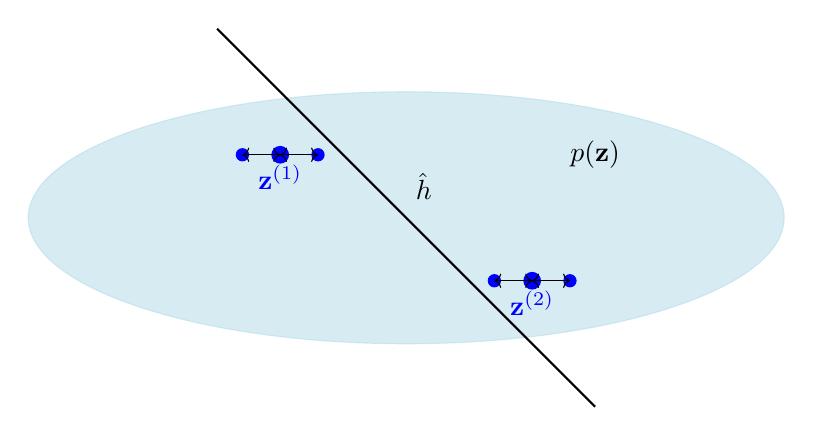
\begin{tikzpicture}[scale=0.8]
 \draw[lightblue, fill=lightblue, opacity=0.5] (3, 2) ellipse (6cm and 2cm);
 \node[black] at (6, 3) {$p({\bf z})$};
 \fill[blue] (1, 3) circle (4pt) node[below, xshift=0pt, yshift=0pt] {${\bf z}^{(1)}$};
 \fill[blue] (5, 1) circle (4pt) node[below] {${\bf z}^{(2)}$};
 \fill[blue] (1.6, 3) circle (3pt);
 \fill[blue] (0.4, 3) circle (3pt);
 \draw[<->, thin] (1, 3) -- (1.6, 3);
 \draw[<->, thin] (1, 3) -- (0.4, 3);
 \fill[blue] (5.6, 1) circle (3pt);
 \fill[blue] (4.4, 1) circle (3pt);
 \draw[<->, thin] (5, 1) -- (5.6, 1);
 \draw[<->, thin] (5, 1) -- (4.4, 1);
 \draw[black, thick, domain=0:6, smooth] plot (\x, {- 1*\x + 5});
 \node[black] at (3, 2.5) [right] {$\hat{h}$};
 \end{tikzpicture}
\end{document}
